\documentclass[]{article}
\usepackage[a4paper, total={15cm,23cm}]{geometry}
\usepackage{fancyhdr}
\usepackage{graphicx}
\usepackage{amsmath}
\usepackage{amssymb}
\usepackage{xcolor}
\usepackage{tikz}
\usepackage{verbatim}
\usepackage{tcolorbox}
\usepackage{textcomp}
\usepackage{xcomment}
\usepackage{xstring}
%opening
\title{PH 223 Week 8}
\author{Benjamin Bauml}
\date{Winter 2024}
\pagestyle{fancy}
\rhead{PH 223}
\chead{Winter 2024}
\lhead{Week 8}

% Version 2024-02-21
% Changes
% 2024-02-21 Added xstring package to enable smooth implementation of new \ModePage command.
% For Assignment, leave Purpose as 1. For Worksheet, set to 2. For Student Solution, set to 3. For Teacher Solution, set to 4.
\newcommand{\Purpose}{1}

\newcommand{\Exclusion}{0}
\newcommand{\PageTurn}{0}
\newcommand{\GrayProb}{0}
\newcommand{\Tipsy}{0}

% Assignment
\if\Purpose1
\renewcommand{\Exclusion}{1}
\fi
% Worksheet
\if\Purpose2
\renewcommand{\Exclusion}{1}
\renewcommand{\PageTurn}{1}
\fi
% Student Solution
\if\Purpose3
\renewcommand{\PageTurn}{1}
\renewcommand{\GrayProb}{1}
\fi
% Teaching Copy
\if\Purpose4
\renewcommand{\PageTurn}{1}
\renewcommand{\GrayProb}{1}
\renewcommand{\Tipsy}{1}
\fi

\if\Exclusion1
\xcomment{Title,Problem,ProblemSub,PassFig}
\fi

\def \NewQ {0}
\def \PForce {0}
\newcommand{\MaybePage}[1]{
	\def \PForce {#1}
	\if\PForce1
		\newpage
	\else
		\if\NewQ0
		\gdef \NewQ {\PageTurn}
		\else
		\newpage
		\fi
	\fi
}

\newcommand{\ModePage}[1]{
	\IfSubStr{#1}{\Purpose}{\newpage}{}
}

\newenvironment{Problem}[2][0]{%The first argument is optional, and if it is set to 1, the \newpage will be forced.
\MaybePage{#1}
\section*{#2}
\if\GrayProb1
\begin{tcolorbox}[colback=lightgray,colframe=lightgray,sharp corners,boxsep=1pt,left=0pt,right=0pt,top=0pt,bottom=0pt,after skip=2pt]
\else
\begin{tcolorbox}[colback=white,colframe=white,sharp corners,boxsep=1pt,left=0pt,right=0pt,top=0pt,bottom=0pt,after skip=2pt]
\fi
}{
\end{tcolorbox}\noindent
}

\newenvironment{ProblemSub}[1][0]{%The argument is optional, and if a string of numbers is entered into it, it will force a \newpage in any \Purpose that shows up in the string. For example, "13" would lead to the newpage being forced in modes 1 and 3.
\ModePage{#1}
\if\GrayProb1
\begin{tcolorbox}[colback=lightgray,colframe=lightgray,sharp corners,boxsep=1pt,left=0pt,right=0pt,top=0pt,bottom=0pt,after skip=2pt]
\else
\begin{tcolorbox}[colback=white,colframe=white,sharp corners,boxsep=1pt,left=0pt,right=0pt,top=0pt,bottom=0pt,after skip=2pt]
\fi
}{
\end{tcolorbox}\noindent
}

\newenvironment{PassFig}{\begin{figure}[h]}{\end{figure}}

\newcommand{\TeachingTips}[1]{
\if\Tipsy1
\begin{tcolorbox}[colback=lightgray,colframe=black]
#1
\end{tcolorbox}
\fi
}

\newenvironment{Title}{\maketitle}{}

\begin{document}
\begin{Title}
\begin{center}
	These problems are borrowed/adapted from Chapters 29 and 30 of the \textit{Student Workbook} for \textit{Physics for Scientists and Engineers}.
\end{center}
\end{Title}

\begin{Problem}{Activity 1}
	(a) Each figure below shows two long straight wires carrying equal currents into or out of the page. At each of the dots, use a \textbf{black} pen or pencil to show and label the magnetic fields $ \vec{B}_{1} $ and $ \vec{B}_{2} $ due to each wire. Then use a {\color{red}\textbf{red}} pen or pencil to show the net magnetic field.
\end{Problem}
\begin{PassFig}
	\centering
	\if\GrayProb1
		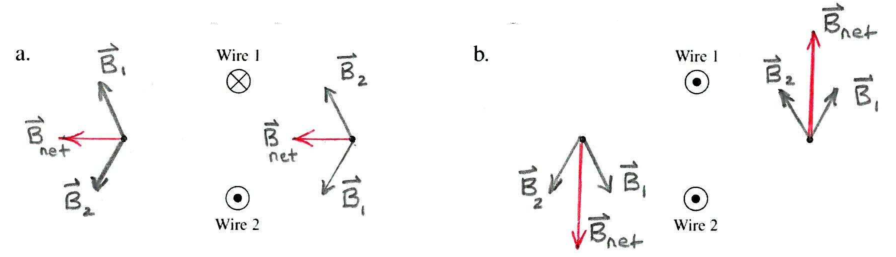
\includegraphics[scale=1]{A1aSol}
	\else
		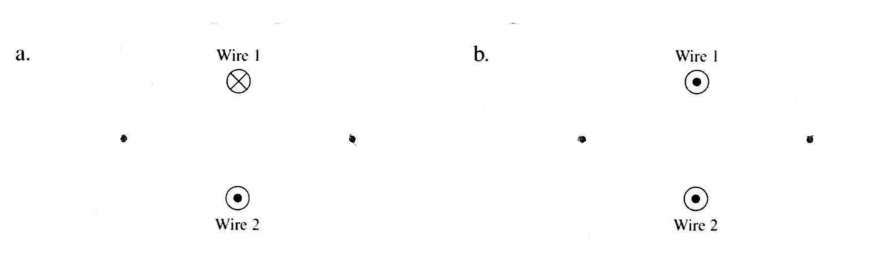
\includegraphics[scale=1]{A1a}
	\fi
\end{PassFig}
\begin{ProblemSub}
	(b) A long, straight wire, perpendicular to the page, passes through a uniform magnetic field. The \textit{net} magnetic field at point 3 is zero. \\
	(i) On the figure, show the direction of the current in the wire. \\
	(ii) Points 1 and 2 are the same distance from the wire as point 3, and point 4 is twice as distant. Construct vector diagrams at points 1, 2, and 4 to determine the net magnetic field at each point.
\end{ProblemSub}
\begin{PassFig}
	\centering
	\if\GrayProb1
	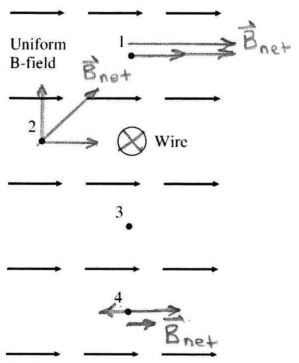
\includegraphics[scale=1]{A1bSol}
	\else
	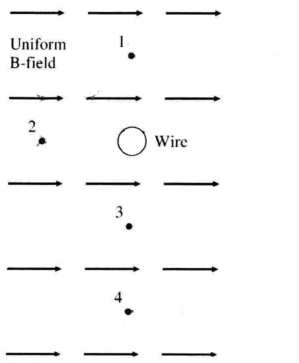
\includegraphics[scale=1]{A1b}
	\fi
\end{PassFig}

\noindent To have a magnetic field around the wire that opposes the uniform field at point 3, the wire must have current into the page. This generates a clockwise magnetic field around the wire. This field has the strength of the uniform field at points 1, 2, and 3, but is upward at 2, and points to the right at 1. At 4, it opposes the uniform field, but it is at half of its strength due to the increased distance.

\begin{Problem}{Activity 2}
	A current-carrying wire passes in front of a solenoid that is wound as shown. The wire experiences an upward force. Use arrows to show the direction in which the current enters and leaves the solenoid. Explain your choice.
\end{Problem}
\begin{PassFig}
	\centering
	\if\GrayProb1
	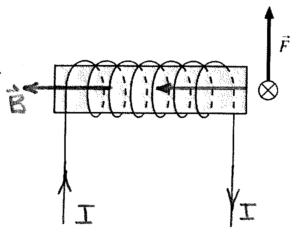
\includegraphics[scale=1]{A3Sol}
	\else
	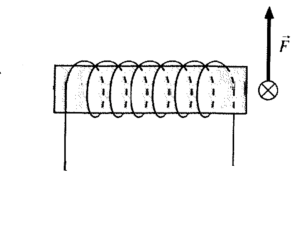
\includegraphics[scale=1]{A3}
	\fi
\end{PassFig}

\noindent To experience an upward force, the straight wire must be in a $ \vec{B} $-field that points to the left. To generate this field in the solenoid, the current direction must be as shown, using the right hand rule.

\TeachingTips{
Especially for this problem, encourage multiple right hand rules (the standard 3-finger vs. the curled fingers).
}

\begin{Problem}{Activity 3}
	The figure shows four circular loops that are perpendicular to the page. The radius of loops 3 and 4 is twice that of loops 1 and 2. The magnetic field is the same for each. Rank in order, from largest to smallest, the magnetic fluxes $ \Phi_{1} $ to $ \Phi_{4} $. Some may be equal.
\end{Problem}
\begin{PassFig}
	\centering
	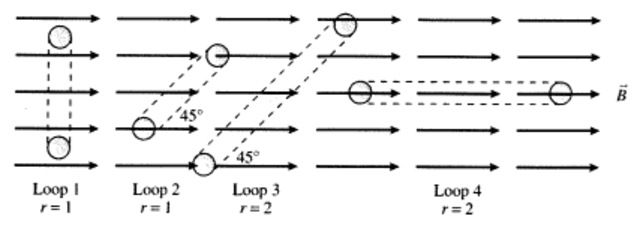
\includegraphics[scale=1]{A1}
\end{PassFig}

\noindent Order: $ \Phi_{3} > \Phi_{1} > \Phi_{2} > \Phi_{4} $ \\
Explanation: In general, flux is calculated as $ \Phi = \int \vec{B}\cdot d\vec{A} $, where the dot product is between the unit normal vector of the plane bounded by the loop and the magnetic field. Since these loops are in a uniform magnetic field, the integration simplifies to a product of the field strength and loop area, multiplied by the cosine of the angle between the normal vector and the magnetic field:
\[
\Phi = AB\cos\theta = \pi r^{2} B\cos\theta.
\]
Let $ r $ be the radius of loops 1 and 2:
\[
\begin{split}
	\Phi_{1} & = \pi r^{2}B\cos(0^{\circ}) = \pi r^{2} B \\
	\Phi_{2} & = \pi r^{2}B\cos(45^{\circ}) = \frac{\pi r^{2} B}{\sqrt{2}} \approx 0.707\Phi_{1} \\
	\Phi_{3} & = \pi (2r)^{2}B\cos(45^{\circ}) = \frac{4\pi r^{2} B}{\sqrt{2}} \approx 2.83\Phi_{1} \\
	\Phi_{4} & = \pi (2r)^{2}B\cos(90^{\circ}) = 0
\end{split}
\]

\TeachingTips{
This activity is actually a bit of a preview, but they should be able to carry over their understanding from electric flux to perform these calculations.
}
\end{document}
